\documentclass[10pt,a4paper,draft]{article}
\usepackage[utf8]{inputenc}
\usepackage{amsmath}
\usepackage{amsfonts}
\usepackage{amssymb}
\usepackage{relsize}
\usepackage{mathtools}
\usepackage[final]{graphicx}
\DeclareMathOperator*{\argmin}{argmin}
\DeclareMathOperator*{\argmax}{argmax}
\newcommand*\perm[2][^n]{\prescript{#1\mkern-2.5mu}{}P_{#2}}
\usepackage{fullpage}
\usepackage{times}
\usepackage{fancyhdr}
\usepackage[ruled,vlined,linesnumbered]{algorithm2e}
\newcommand\mycommfont[1]{\footnotesize\ttfamily\textcolor{blue}{#1}}
\SetCommentSty{mycommfont}
\usepackage{xcolor}

\usepackage{csvsimple}
\usepackage{booktabs}
\usepackage{longtable}
\usepackage{pgfplotstable}
\pgfplotsset{compat=1.9}% supress warning

\begin{document}
\title{RL Approach for the TSP Problem}
\author{Avrech Ben-David}
\maketitle
\begin{abstract}
In this work we review the recent works in this field. Our purpose is to point on an optional improvement direction which has not been investigated yet, and which we think has a good potential. 
\end{abstract}
\section{Introduction}
The TSP problem is a fundemental NP-hard combinatorial problem with myriad applications in the industry. Recently, many RL approaches were investigated in order to learn an efficient heuristic to solve the TSP problem. A probable reason is that many variations of the TSP problem can be simply formulated in RL terms, saving the costly development time of ad-hoc solvers. 

However, when testing the generalization ability, there is still a gap of approximately 10\% in performance between all these approaches and the best known solver \cite{concorde}, Concorde. Concorde has time complexity of $\mathcal{O}(n^22^n)$ in the worst case, but in the average case it solves instances of thousands of cities to optimality in minutes. The main weakness of Concorde is that it able to solve only the symmetric TSP. 

There is already a success in applying RL to NP-hard combinatorial problems (MVC, SCP, MAXCUT - see \cite{dai17-tsp-s2v}), but the common characteristic of all these 'solved' problems is that they are all \textit{n-choose-k}-like problems. \cite{dai17-tsp-s2v} solve MVC, SCP and MAXCUT to 1\% from the optimal, generalize well and consume much less computation resources than competitive solutions. However, they fail in the TSP. Other works, \cite{bello16-tsp-pnac} and \cite{deudon18-tsp-nr2opt}, use Pointer Networks to solve the TSP. All these works solve the instance they were trained on plausibly, but they fail to generalize to larger instances. While \cite{dai17-tsp-s2v} maintain an approximation ratio of 1.1 on a large scale of graphs (up to 1K nodes), the others fail to generalize to more than 100 nodes. 

In this work we follow \cite{dai17-tsp-s2v}, investigating their weaknesses, in order to predict a probably good improvement.

\section{Related Work}
\cite{bello16-tsp-pnac} were the train locomotive in using Pointer Networks to parameterize a stochastic policy of selecting nodes into the TSP solution. They proposed the common RL formulation for the TSP; the state is the current partial solution - an ordered list of nodes; the action is appending a node to the end of the tour; and the reward is the final tour length. They parameterized the target policy by LSTM-based pointer network, and trained it with REINFORCE-Actor-Critic, to predict a sequence of nodes one by one. They used Monte-Carlo estimator for the reward signal as it is the natural choice for the TSP, where the total reward can extremely change in the final step. Their architecture is limited to fully-connected graphs in the 2D Euclidean space, and requires a long training time. They fail in handling large instances (more than 100 nodes).

\cite{deudon18-tsp-nr2opt}, following \cite{bello16-tsp-pnac}, replaced the LSTMs with feed forward components, leaving the pointing mechanism as is. The decoder, composed of a pipeline of 3 stages, explicitely forgets after three steps. The other RL settings remained the same. Obviously, this simplified implementation achieved poor performance by its own, and for this they used 2opt, a local search algorithm to refine the solution. At the bottom line, they improved the performance of \cite{bello16-tsp-pnac} insignificantly, while reducing the model size and the training time dramatically. Anyway, they suffer from the same poor generalization, and the inference time become very long on large graphs due to the 2opt search.

A completely different approach was proposed by \cite{dai17-tsp-s2v}. They used S2V \cite{dai16-s2v} to represent the graph nodes, and learned a Q-function over these features. They trained the network end to end, via a so called n-step-DQN algorithm (see alg below). Their state is the current partial solution, the action is inserting a node to the partial solution such that the increase in the total length is minimal. The reward is the negative increase in the tour length after taking the action. Their architecture can easily handle any graph structure, and maintain performance on much larger graphs than it was trained on. 

The first and repairable problem is that the Q-function averages the nodes features, throwing away the information of the nodes order. This problem can be viewed in the order the network selects nodes to the partial solution. The network was probably planned to address the mentioned \textit{n-choose-k}-like problems, which are insensitive to the nodes prediction order.

The second and more problematic issue is the reward definition. It is not clear if even n-step reward is good enough to evaluate an action quality. As mentioned, the TSP solution cost can extremely grow in the final step, when closing the loop.

Following, in Section \ref{sec-methodology} we describe the solution in detail. First we define the RL formulation for the TSP. Next we give an introduction to the network components. The training process is explained in Section \ref{sec-training}. We detail our experimental setup and results in Section \ref{sec-experiments}. In Section \ref{sec-conclusions} we discuss our findings, and highlights the weaker elements in this work. Finally we offer a future work in Section \ref{sec-roadmap}.

\section{Methodology} \label{sec-methodology}
\subsection{Problem Statement}
The traveling salesman problem is: given a graph $G(V,E)$, find the visiting order, such that every node in $V$ is visited exactly once, and the total length of the circular tour is minimal. Representing the graph nodes as a list: $V = \{1,2,3,...,n\}$, the TSP solution $S$ is a permutation of $V$, such that:

\begin{equation} \label{tsp_statement}
	S = \argmin_{s \in Perm(V)} C(S)
\end{equation}

Where $C(S)$ is the TSP cost function - i.e. the tour length:

\begin{equation}  \label{tsp_cost}
	C(S) := \mathlarger{\sum}_{i=1}^{|S|}{distance(s_i, s_{i+1})} + distance(s_{|S|}, s_1)
\end{equation}

In the classic TSP, the $distance(\cdot,\cdot)$ can be any metric that preserve the triangle inequality. Here we deal only with the 2D Euclidean distance. 

\subsection{TSP RL Formulation}	
The TSP naturally lands to the RL standard formulation, mainly because the final $reward$ is well defined in the TSP statement itself. 
\cite{dai17-tsp-s2v} use DQN with \textit{experience replay} with n-step reward (see alg below). The MDP is defined as follows:
\begin{list}{}{}
	\item[•] State $s_t$ - An ordered sequence of $t$ selected nodes $\in \perm[n]{t}$, representing the current partial solution. The environment is initialized with empty solution $s_0 = \{\}$.
	\item[•] Action $a_t(v)$ - Adding a node $v \not\in S(k)$ to the partial solution, and placing it greedily to minimize the increase in the tour length $C(S)$. Adding a node inherently defines the transition from state $s_t$ to $s_{t+1}$.
	\item[•] Reward $r(s_t,a_t)$ - The change in the cost function, after taking action $a_t$ in the state $s_t$ and transitioning to state $s_{t+1}$, i.e. $C(s_{t+1})-C(s_t)$. The accumulated reward over $n$ steps $r_t^{(n)}$ is the total increase $C(s_{t+n})-C(s_t)$. The final reward of an episode is the total tour length $C(s_{|V|})$
\end{list}


\subsection{Q Network}
We follow S2V paradigm of approximating the State-Action value function.
Designing the $Q$ function is our main task. S2V-DQN uses a permutation invariant function, in the meaning that it averages the graph nodes features. Probably it was designed at first for permutation-agnostic problems, such as MVC. Our desired is a $Q$ function that is sensitive to the visiting order of the nodes, but must not overfit to specific input order. 

\cite{dai17-tsp-s2v} propose the following parameterization for $Q(s,a)$:
First, at the begining of every state, we update the S2V embeddings, by running $T$ iterations of massage passing:
\begin{equation}
	\mu_v^{(t+1)} \leftarrow Relu\Bigg(\theta_1 x_v + \theta_2 \sum_{u \in \mathcal{N}(v)} \mu_u^{(t)} + \theta_3 \sum_{u \in \mathcal{N}(v)} Relu\big(\theta_4 w(v,u)\big)\Bigg)
		\label{s2v-dqn-nodes-features}
\end{equation}

After embedding the current state $s_t$, we use $\widehat{Q}(s,a;\theta)$ to predict the value of an optional action:
\begin{equation}
	Q(s,a;\theta) = \theta_5^\top Relu\bigg(concat\big(\theta_6 \sum_{v \in V} \mu_v^{(T)}, \theta_7 \mu_a^{(T)}\big)\bigg)
	\label{s2v-dqn-qfunc}
\end{equation}

\subsection{Q Learning}
We use here a modified DQN algorithm. In the basic DQN we use the same Q architecture for the $\varepsilon-greedy$ behavior policy $\pi_b(a|s)$ and the $greedy$ target policy $\pi^*(a|s)$.

\begin{equation}
\pi^*(a|s) = \argmax_{a \notin s}{Q^*(s,a;\theta^-)}
\label{dqn-target-policy}
\end{equation}

\begin{equation}
\pi_b(a|s) = 
\begin{dcases}
    random \ {a \notin s} 					& \text{w.p  \ \ } \varepsilon \\
    \argmax_{a \notin s}{Q(s,a;\theta)} 	& \text{otherwise}
\end{dcases}
\label{dqn-behavior-policy}
\end{equation}
We use the behavior policy, parameterized by $\theta$ to select an action $a_t$ for the current state $s_t$, and the target policy, parameterized by $\theta^-$ for estimating the DQN target, originally defined as:
\begin{equation}
y_t = r_t + \gamma\max_{a'}Q(s_{t+1},a';\theta^-)
\label{orig-dqn-target}
\end{equation}
The only modification is that we use the sum of the following $n$ rewards $r_t^{(n)} = \sum_{i=0}^{n-1} r_{t+i}$, and after that bootstrap using the target policy \eqref{dqn-target-policy}:
\begin{equation}
y_t = r_t^{(n)} + \gamma\max_{a'}Q(s_{t+n},a';\theta^-)
\label{s2vdqn_target}
\end{equation}
The objective function at step $t$ is the squared error between the target and the learned $Q$ function:
\begin{equation}
L_t(\theta) = \big(y_t - Q(s_t,a_t;\theta)\big)^2
\label{dqn_objective}
\end{equation}
We can now optimize this loss w.r.t $\theta$ using SGD. In order to reduce the updates variance, DQN use an \textit{experience-replay}. We retroactivelly store each state-action pair with its following accumulated rewards, and the resultant state $<s_t, a_t, r_t^{(n)}, s_{t+n}>$ in a replay memory $\mathcal{M}$. At each update we sample a batch of examples $\mathcal{B} ~^{i.i.d} \mathcal{M}$ and make a more stable update of $\theta$. The target parameters $\theta^-$ are updated every certain number of steps by $\theta$ to prevent chase after a moving target.

The learning process is detailed in algorithm \eqref{s2v-dqn-alg}.


\begin{algorithm}[H]
	\SetAlgoLined
	\DontPrintSemicolon
	\KwResult{$\theta$}
 	Initialize replay memory $\mathcal{M}$ to capacity $N$ \\
	Initialize agent network parameters $\theta$ \\
	Initialize target network parameters $\theta^- \leftarrow \theta$ \\
	Set target update period $T_{update}$ \\ 
	Set global counter $t_{global} = 1$ \\
	\For{episode 1 to L}{
		Initialize environment and state $s_0$ \\
		\For{step t = 1 to T}{
			select action $a_t$ according to \eqref{dqn-behavior-policy} \\
			observe reward $r_t$ and new state $s_{t+1}$ \\
			\If{$t \geq n$}{			
				$r_{t-n+1}^{(n)} \leftarrow \mathlarger{\sum}_{i=0}^{n-1} \gamma^i r_{t-n+1+i}$  \tcp*{last n-steps reward} 
				store $<s_{t-n+1}, a_{t-n+1}, r_{t-n+1}^{(n)},s_{t+1}>$ in $\mathcal{M}$ \\
				sample a random mini-batch $\mathcal{B} \stackrel{i.i.d}{\sim} \mathcal{M}$ \\
				\For{$<s_j, a_j, r_j^{(n)}, s_{j+n}>$ in $\mathcal{B}$}{
					$y_j \leftarrow 
						\begin{dcases}
					    r_j^{(n)}				& \text{for terminal } s_{j+n} \\
					    r_j^{(n)} + \gamma^n \max_{a'}Q(s_{j+n},a';\theta^-) 	&  \text{for non-terminal } s_{j+n}
						\end{dcases} 
					$ \tcp*{calculate target}
					$L_j(\theta) \leftarrow \big(y_j - Q(s_j,a_j;\theta)\big)^2$ \tcp*{calculate loss} 
				}
				perform SGD on $L_j(\theta)$ \\
			}
		}
		\If{$t_{global} \mod T_{update} == 0$}{
			$\theta^- \leftarrow \theta$	\tcp*{update target parameters}		
		}
		$t_{global} \leftarrow t_{global} + 1$
	} 
	\caption{S2V-DQN: n-step reward with Experience Replay}
 	\label{s2v-dqn-alg}
\end{algorithm}

Now we can conceptually optimize our network end-to-end.

\section{Training Setup} \label{sec-training}
The network parameterization details are as in \cite{dai17-tsp-s2v}, and only the hyper-parameters were changed. Apart of the original setup: $\gamma=0.1, \varepsilon \equiv 1, l2=0$ and \textit{n-step} $=1$, we further experimented with a large scale of these parameters, in order to understand the network behavior. In spite of the competitive performance of the network, comparing to other works, the original parameters values do not make sense, and the authors do not supply convincing explanation.

The training process is as follows:
\begin{list}{•}{•}
	\item Training starts with 1000 exploration episodes with $\varepsilon = 1$
	\item The target parameters are updated every 1000 behavior updates
	\item $\varepsilon1$ is decayed almost linearly from a specified initial value, to a constant final value
	\item The learning rate is multiplied by 0.95 every 1000 behavior updates
	\item The network is evaluated every 100 episodes on a held-out validation set, and the parameters are stored with the average tour length
	\item The final parameters are selected to minimize the validation average tour length
\end{list}

\section{Experiments} \label{sec-experiments}
\subsection{Baselines}	
We use Concorde\footnote{https://github.com/jvkersch/pyconcorde} to compute the optimal solution. We report approximation ratio and execution time ratio comparing to the optimal solution. The ratio is defined as $\dfrac{Model_{performance}}{Concorde_{performance}} $ so as the ratio is closer to 1 the tested model is better.
As an on-the-shelf algorithm, we used cross-entropy method\footnote{https://github.com/v-iashin/CrossEntropyTSP}, note that it certainly emphasises the necessity of smart solver.
We trained and evaluated the network of \cite{deudon18-tsp-nr2opt}, which we refer to as nr2opt, using their original data generator. We compared the generalization ability of nr2opt to S2V-DQN, and show that S2V-DQN outperforms \cite{deudon18-tsp-nr2opt} even in case it was trained on much smaller graphs and on different data distribution.

\subsection{Realworld Data - Experimental Setup} \label{realworld-exp}
The results below refer to the Tsplib dataset\footnote{http://dimacs.rutgers.edu/Challenges/TSP/}. The dataset contains 38 cities of 51-318 nodes each one.
In this experiment	S2V-DQN was trained for 100,000 epochs on a single sample (berlin52). We used the original network hyper-parameters.
Table \ref{tb_tsplib_performance_s2v_vs_ce} shows the approximation ratio per execution time ratio of S2V-DQN comparing to cross-entropy method. The cross-entopy method was too slowly on larger graphs, and anyway, we find it sufficient to report onlt this small sample of cities.
	
	\begin{table}[h] \centering
	\begin{tabular}{lll}
	 	Instance Name	& S2V   		& Cross-Entropy Method 	\\
	 	berlin52 		& 1.007@1.47	& - 					\\
		eil51  			& 1.049@1.73	& 1.16@5075				\\
		st70 			& 1.065@1.56 	& 1.17@16666 			\\
		eil76			& 1.066@3.45 	& 1.12@31000
	\end{tabular}
	\caption{Tsplib Small Cities Approximation Ratio per Time Ratio} 
	\label{tb_tsplib_performance_s2v_vs_ce}
	\small S2V-DQN trained on berlin52 for 100,000 epochs. The logic behind training S2V-DQN on a single instance\footnote{This was the answer I got for why did they trained the model on a single city only.} is demonstrating the ability of S2V-DQN to solve TSP as an out-of-the-box solver, exactly as we use cross-entropy method as an on-the-shelf solver. The cross-entropy methods takes 11 minutes to solve 52 nodes, and it seems like it grows exponentially.
	\end{table}

 

\subsection{Synthetic Data Experiment}
In order to understand the contribution of the training set to the test results, we trained S2V-DQN on a synthetic dataset\footnote{https://www.dropbox.com/sh/r39596h8e26nhsp/AADRm5mb82xn7h3BB4KXgETsa?dl=0}, consists of either clustered or uniformly distributed graphs. The model was trained on 1000 graphs of 15-20 nodes. We observed that the performance is the same as if we trained the network on a single instance as in section \ref{realworld-exp}. The average approximation ratio over the entire Tsplib dataset was 1.092, and the execution time ratio was 0.91. It seems that this performance level really reflects the S2V architecture expressiveness. We assert this declaration in an exhaustive experiment as described in section \ref{exhaustive-search-exp}.

\subsection{Exhaustive Search Experiment} \label{exhaustive-search-exp}
\cite{dai17-tsp-s2v} reported weired hyper-parameters selection, which arises questions about the model ability to learn the TSP. The original parameter-set was $\{\gamma=1, \varepsilon=1 \text{(without decay at all)}, l2=0, nstep=1\}$. $\gamma=1$ defines almost totaly greedy policy, regardless of the tracked \textit{n-steps}, and explicitely does not fit the TSP nature. 

In order to understand the model weaknesses better, we performed an exhaustive search on a large scale of parameters and evaluated the model on a slightly different data distribution. S2V-DQN was trained on synthetic clustered graphs in $[0,1]^2$, and evaluated on uniformly distributed graphs of 100 and 200 nodes supplied by \cite{deudon18-tsp-nr2opt}.

We also compared the results to \texttt{nr\_only}, the pointer network proposed by \cite{deudon18-tsp-nr2opt}, trained from scratch using it's original setup. S2V-DQN outperforms \cite{deudon18-tsp-nr2opt} even "in their home". Following,  \texttt{nr\_only} and \texttt{nr2opt} refer to the pointer network alone, and to the setup which it is followed by 2opt refinement.

\begin{table}[]
\centering
\begin{tabular}{@{}llllllll@{}}
\toprule
Model           & Trained on          & Nstep      & $\gamma$     & $\varepsilon$   & l2            & Approximation  & Time            \\ \midrule
\textbf{nr2opt} & \textbf{50}         & \textbf{-} & \textbf{-}   & \textbf{-}      & \textbf{-}    & \textbf{1.061} & \textbf{18.826} \\
\textbf{S2V}    & \textbf{rand-40-50} & \textbf{1} & \textbf{0.1} & \textbf{1-to-1} & \textbf{0.00} & \textbf{1.081} & \textbf{1.070}  \\
S2V             & clus-15-20          & 5          & 0.9          & 1-to-0.1        & 0.00          & 1.084          & 1.102           \\
S2V             & clus-15-20          & 4          & 0.9          & 1-to-1          & 0.00          & 1.084          & 1.154           \\
S2V             & clus-15-20          & 5          & 0.9          & 1-to-1          & 0.00          & 1.084          & 1.118           \\
S2V             & clus-15-20          & 7          & 0.1          & 1-to-0.1        & 0.0001        & 1.085          & 1.115           \\
S2V             & clus-15-20          & 2          & 0.9          & 1-to-0.1        & 0.00          & 1.085          & 1.030           \\
S2V             & clus-15-20          & 4          & 0.9          & 1-to-0.1        & 0.00          & 1.085          & 1.005           \\
S2V             & clus-15-20          & 3          & 0.9          & 1-to-1          & 0.00          & 1.085          & 1.012           \\
S2V             & clus-15-20          & 4          & 0.9          & 1-to-1          & 0.0001        & 1.086          & 1.121           \\
S2V             & clus-15-20          & 3          & 0.9          & 1-to-0.1        & 0.00          & 1.086          & 1.104           \\
S2V             & clus-15-20          & 2          & 1            & 1-to-0.1        & 0.0001        & 1.087          & 1.010           \\
S2V             & clus-15-20          & 3          & 0.1          & 1-to-1          & 0.00          & 1.087          & 0.971           \\
S2V             & clus-15-20          & 2          & 0.9          & 1-to-0.1        & 0.0001        & 1.089          & 1.051           \\
S2V             & clus-15-20          & 2          & 1            & 1-to-1          & 0.0001        & 1.089          & 1.028           \\
S2V             & clus-15-20          & 3          & 0.1          & 1-to-1          & 0.0001        & 1.090          & 1.082           \\
S2V             & clus-40-50          & 3          & 1            & 1-to-0.01       & 0.00          & 1.094          & 1.280           \\
S2V             & clus-40-50          & 6          & 1            & 1-to-0.01       & 0.00          & 1.096          & 1.053           \\
S2V             & clus-15-20          & 3          & 0.9          & 1-to-1          & 0.0001        & 1.100          & 1.013           \\
S2V             & clus-15-20          & 4          & 1            & 1-to-1          & 0.0001        & 1.115          & 1.076           \\
S2V             & clus-15-20          & 4          & 0.9          & 1-to-0.1        & 0.0001        & 1.123          & 1.018           \\
S2V             & clus-15-20          & 7          & 1            & 1-to-0.1        & 0.0001        & 1.126          & 1.108           \\
S2V             & clus-15-20          & 7          & 0.9          & 1-to-0.1        & 0.0001        & 1.128          & 0.960           \\
S2V             & clus-15-20          & 4          & 1            & 1-to-0.1        & 0.0001        & 1.138          & 1.033           \\
nr\_only        & 50                  & -          & -            & -               & -             & 1.175          & 0.778           \\ \bottomrule
\end{tabular}
\caption{Exhaustive Search Results on Random Graphs of 100 Nodes}
\label{exhastive-search-results100}
\end{table}
    
% Please add the following required packages to your document preamble:
% \usepackage{booktabs}
\begin{table}[]
\centering
\begin{tabular}{@{}llllllll@{}}
\toprule
\textbf{Model} & \textbf{Trained on} & \textbf{Nstep} & \textbf{gamma} & \textbf{epsilon} & \textbf{l2} & \textbf{Approx} & \textbf{Time} \\ \midrule
\textbf{S2V} & \textbf{rand-40-50} & \textbf{1} & \textbf{0.1} & \textbf{1-to-1} & \textbf{0.00} & \textbf{1.095} & \textbf{0.825} \\
S2V & clus-15-20 & 4 & 0.9 & 1-to-1 & 0.00 & 1.098 & 0.816 \\
S2V & clus-15-20 & 7 & 0.1 & 1-to-0.1 & 0.0001 & 1.099 & 0.836 \\
S2V & clus-15-20 & 2 & 1 & 1-to-1 & 0.0001 & 1.100 & 0.827 \\
S2V & clus-15-20 & 2 & 0.9 & 1-to-0.1 & 0.0001 & 1.100 & 0.794 \\
S2V & clus-15-20 & 2 & 1 & 1-to-0.1 & 0.0001 & 1.100 & 0.902 \\
S2V & clus-15-20 & 3 & 0.9 & 1-to-0.1 & 0.00 & 1.100 & 0.817 \\
S2V & clus-15-20 & 4 & 0.9 & 1-to-0.1 & 0.00 & 1.101 & 0.872 \\
S2V & clus-15-20 & 2 & 0.9 & 1-to-0.1 & 0.00 & 1.103 & 0.786 \\
S2V & clus-40-50 & 3 & 1 & 1-to-0.01 & 0.00 & 1.103 & 0.853 \\
S2V & clus-40-50 & 6 & 1 & 1-to-0.01 & 0.00 & 1.104 & 0.805 \\
S2V & clus-15-20 & 4 & 0.9 & 1-to-1 & 0.0001 & 1.104 & 0.828 \\
S2V & clus-15-20 & 3 & 0.1 & 1-to-1 & 0.00 & 1.104 & 0.818 \\
S2V & clus-15-20 & 3 & 0.1 & 1-to-1 & 0.0001 & 1.105 & 0.819 \\
S2V & clus-15-20 & 3 & 0.9 & 1-to-1 & 0.0001 & 1.123 & 0.762 \\
S2V & clus-15-20 & 4 & 0.9 & 1-to-0.1 & 0.0001 & 1.134 & 0.768 \\
S2V & clus-15-20 & 7 & 1 & 1-to-0.1 & 0.0001 & 1.135 & 0.805 \\
S2V & clus-15-20 & 4 & 1 & 1-to-1 & 0.0001 & 1.141 & 0.758 \\
S2V & clus-15-20 & 4 & 1 & 1-to-0.1 & 0.0001 & 1.158 & 0.837 \\
S2V & clus-15-20 & 7 & 0.9 & 1-to-0.1 & 0.0001 & 1.176 & 0.792 \\
nr2opt & 50 & - & - & - & - & 1.571 & 0.879 \\
nr\_only & 50 & - & - & - & - & 1.602 & 0.392 \\ \bottomrule
\end{tabular}
\caption{Exhaustive Search Results on Random Graphs of 200 Nodes}
\label{exhastive-search-results200}
\end{table}

Tables \ref{exhastive-search-results100} and \ref{exhastive-search-results200} lists the parameters grid search. Note that \texttt{nr\_only} by itself has poor peformance, and \texttt{nr2opt} execution time is much higher that Concorde. On 200 nodes \cite{deudon18-tsp-nr2opt} is out of the game. The results assert that the original S2V-DQN parameters of \cite{dai17-tsp-s2v} are the best choice. it strengthens the hypothesis that either the architecture or the reward estimation do not fit the TSP.

\subsection{Results from the Original Paper}
Figure \ref{im_paper_aprx_comp} gives an overview of the existing approaches, due to 2016. For more analyses and approximation-time trade-off refer to \cite{dai17-tsp-s2v}. There is no heuristic that generalizes better than S2V-DQN, and all of them are bounded to 9-10\% from the optimal. The performance do not improve if we train S2V-DQN on large graphs, as can be depicted from figure \ref{im_paper_aprx_vs_trainsize}.

\begin{figure}[h]
	\centering
	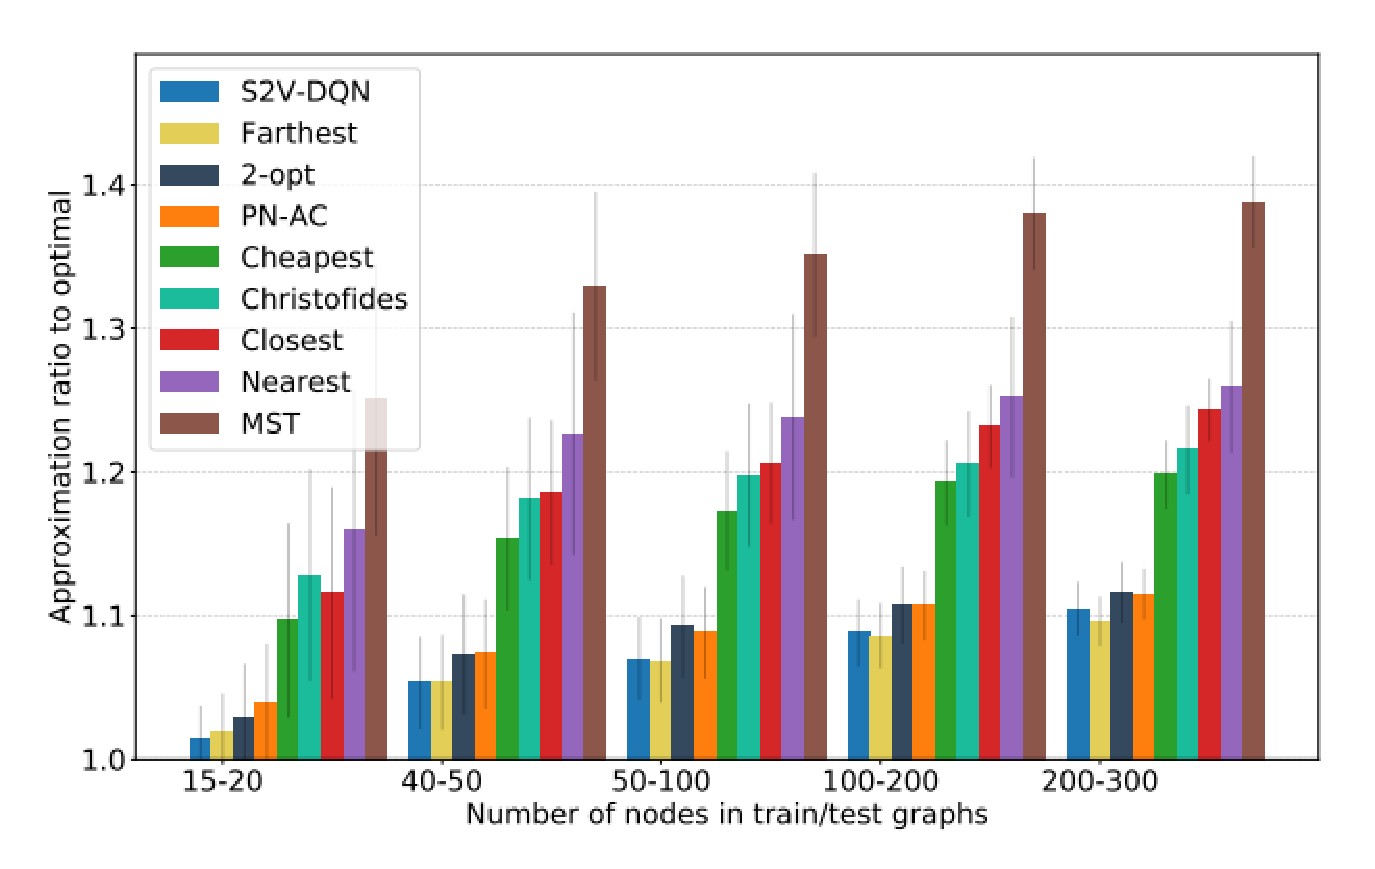
\includegraphics[width=1\textwidth]{tsp_paper_res_comp.eps}	
	\medskip
	\caption{Comparison of Existing Approaches to the TSP}
	\small On large instances S2V-DQN is not better than others in terms of approximation ratio.
	\label{im_paper_aprx_comp}
\end{figure}
\begin{figure}[h]
	\centering
	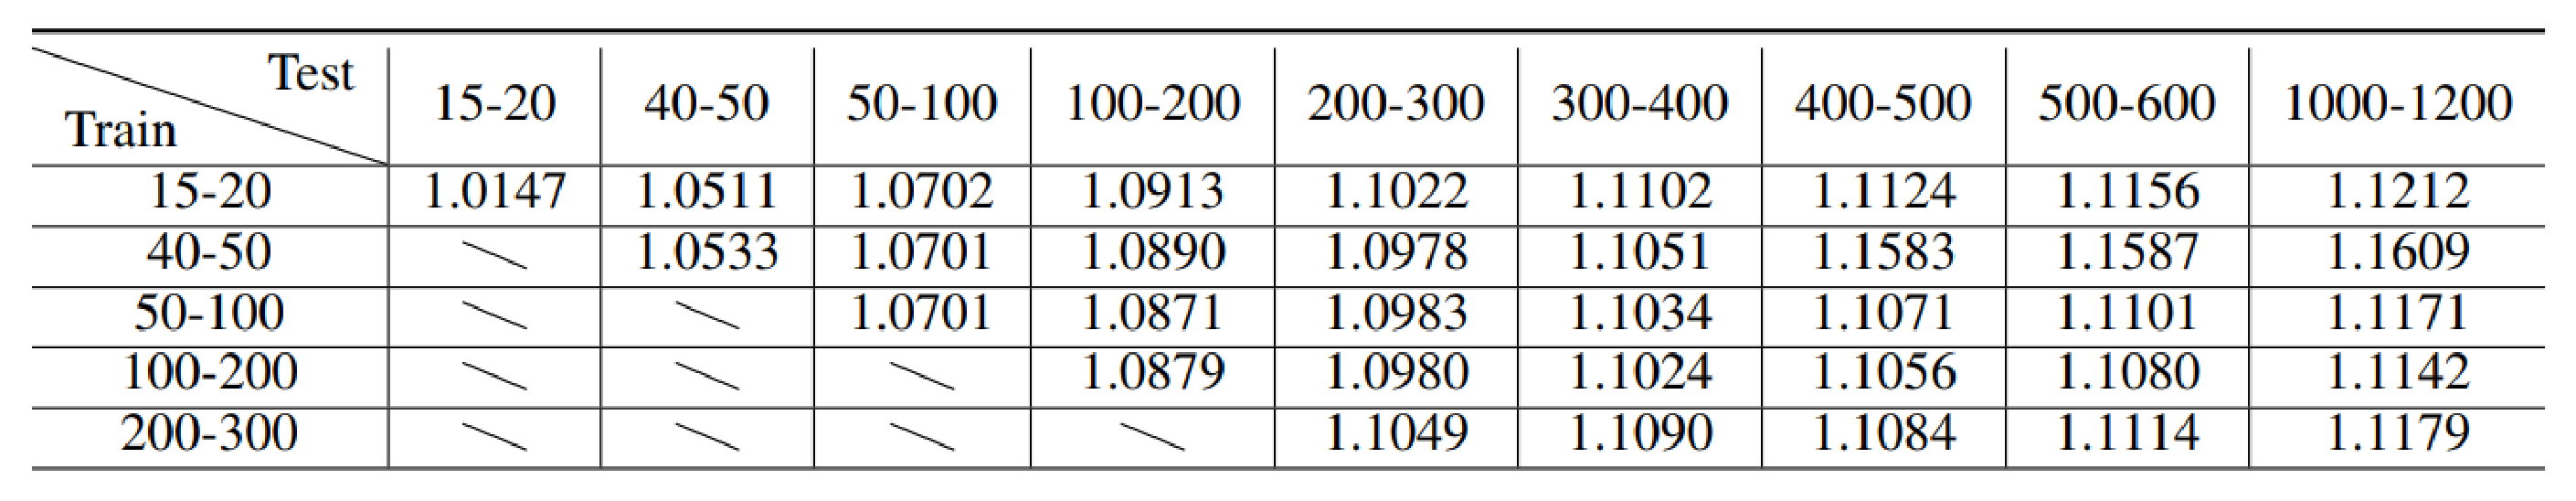
\includegraphics[width=1\textwidth]{tsp_paper_res_table.eps}
	\caption{S2V-DQN Generalization as function of Training Graphs Size}
	\small No matter how much you train, the approximation ratio remains the same.
	\medskip
	\label{im_paper_aprx_vs_trainsize}
\end{figure}	

	
\section{Conclusions} \label{sec-conclusions}
The authors explained the fact that S2V did not show impressive performance on the TSP problem in that the tested graphs are fully-connected. The graph structure is less important, and even "graph-agnostic" methods achieve the same performance. This answers why other proposals show comparable results to S2V-DQN, but it does not answer why all of the results degrades with the graph size.

We highlight two important weaknesses: 1. The Q netowrk architecture, 2. The reward estimation.
1. The S2V-DQN architecture has a built-in disadvantage regarding sequence mapping. Averageing the nodes features in \ref{s2v-dqn-qfunc} ignores the state essential information about the current tour. Originally, the nodes features were summed  in order to be invariant to permutations. It works well on MVC and probably on any other ${n \choose k}$-like problem.

2. Actually, S2V-DQN performs its best when configured to learn a completely greedy policy. Setting $\gamma=0.1$ actually ignored the delayed reward, and makes the \textit{n-step} property useless. The fact that setting high values of $\gamma$ and \textit{n-step} do not show improvement can derive from two reasons:
The first is that \textit{n-step} learning might not be sufficient in the TSP, because the reward can dramatically change in the last steps of an episode. Moreover, using the negative increase in tour as the immediate reward biases the policy to greedy steps. It is certainly the easy way to define the reward but it absolutely contradicts the TSP intuition.

The second is the problematic architecture of $Q(s,a;\theta)$. This is certainly changeable, and there is only one way to assess this hypothesis, testing it.

Another weird setting is the obssession of exploration. Setting $\varepsilon$ to 1 constantly, implies that we do not trust the learned policy at all. Does the learnd policy so arbitrary? If so, why do we spend so much efforts on RL?
\section{Roadmap} \label{sec-roadmap}
As a first step we have to implement S2V-DQN in pure Python and restore the original results. It might take 2-3 months. The second step is to change the $Q$ parameterization.
Further research would investigate the reward estimation, e.g Monte Carlo reward estimator. Other RL methods, say, policy gradient methods, are also an option, but eventually, all of these methods are the same same.

\bibliography{tsp-rl-report}
\bibliographystyle{plain}
\end{document}